%%%%%%%%%%%%%%%%%%%%%%%%%%%%%%%%%%%%%%%%%%%
%
% From a template maintained at https://github.com/jamesrobertlloyd/cbl-tikz-poster
%
%%%%%%%%%%%%%%%%%%%%%%%%%%%%%%%%%%%%%%%%%%%


\documentclass[portrait,a0b,final,a4resizeable]{include/a0poster}


\usepackage{multicol}
\usepackage{color}
\usepackage{morefloats}
\usepackage[pdftex]{graphicx}
\usepackage{rotating}
\usepackage{amsmath, amsthm, amssymb, bm}
\usepackage{array}
\usepackage{booktabs}
\usepackage{multirow}
\usepackage{hyperref}


\usepackage{include/picins}
\usepackage{tikz}
\usetikzlibrary{shapes.geometric,arrows,chains,matrix,positioning,scopes,calc}
\tikzstyle{mybox} = [draw=white, rectangle]
\definecolor{darkblue}{rgb}{0,0.08,0.45}
\definecolor{blue}{rgb}{0,0,1}



%\usepackage{nicefrac}
%\newcommand{\vect}[1]{\underline{\smash{#1}}}
%\renewcommand{\v}[1]{\vect{#1}}
%\newcommand{\reals}{\mathds{R}}
%\newcommand{\sX}{\mathcal{X}}
%\newcommand{\sD}{\mathcal{D}}
%\newcommand{\br}{}%{^{\text{\textnormal{ r}}}}
%\newcommand{\cat}{^{\text{\textnormal{c}}}}

\usepackage{dsfont}

%\ProvidesPackage{preamble}

\usepackage{url}
\usepackage{array}
\usepackage{amsmath,amssymb,amsfonts,textcomp,amsthm}
\usepackage{booktabs}
\usepackage{relsize}
\usepackage{nicefrac}
\usepackage{graphicx}
\usepackage{rotating}
\usepackage{nth}
\usepackage{acronym}
\usepackage{bm}
%\usepackage{caption} \DeclareCaptionType{copyrightbox}
\usepackage{footnote}
\usepackage{color}

\usepackage{tabularx}
\newcolumntype{x}[1]{>{\centering\arraybackslash\hspace{0pt}}m{#1}}
\newcommand{\tabbox}[1]{#1}

\usepackage{hyperref}
\definecolor{mydarkblue}{rgb}{0,0.08,0.45}
\hypersetup{
    pdftitle={},
    pdfauthor={},
    pdfsubject={},
    pdfkeywords={},
    pdfborder=0 0 0,
    pdfpagemode=UseNone,
    colorlinks=true,
    linkcolor=mydarkblue,
    citecolor=mydarkblue,
    filecolor=mydarkblue,
    urlcolor=mydarkblue,
    pdfview=FitH}

\newcommand{\asdf}{$^{\textnormal{th}}$}

\newcommand{\binarysum}{\sum_{\bf{x} \in \{0,1\}^D}}
\newcommand{\expect}{\mathbb{E}}
\newcommand{\expectargs}[2]{\mathbb{E}_{#1} \left[ {#2} \right]}
\newcommand{\var}{\mathbb{V}}
\newcommand{\varianceargs}[2]{\mathbb{V}_{#1} \left[ {#2} \right]}
\newcommand{\variance}{\mathbb{V}}
\newcommand{\cov}{\operatorname{cov}}
\newcommand{\Cov}{\operatorname{Cov}}
\newcommand{\covarianceargs}[2]{\Cov_{#1} \left[ {#2} \right]}
\newcommand{\colvec}[2]{\left[ \begin{array}{c} {#1} \\ {#2} \end{array} \right]}
\newcommand{\tbtmat}[4]{\left[ \begin{array}{cc} {#1} & {#2} \\ {#3} & {#4} \end{array} \right]}

%\newcommand{\covskinny}[2]{\var\!\left(#1\middle\vert#2\right)} 

\newcommand{\acro}[1]{\textsc{#1}}
%\newcommand{\vect}[1]{\boldsymbol{#1}}
\newcommand{\vect}[1]{{\bf{#1}}}
\newcommand{\mat}[1]{\mathbf{#1}}
\newcommand{\pderiv}[2]{\frac{\partial #1}{\partial #2}}
\newcommand{\npderiv}[2]{\nicefrac{\partial #1}{\partial #2}}

\newcommand{\pha}{^{\phantom{:}}}

\newcommand{\argmin}{\operatornamewithlimits{argmin}}
\newcommand{\argmax}{\operatornamewithlimits{argmax}}

% The following designed for probabilities with long arguments

\newcommand{\Prob}[2]{P\!\left(\,#1\;\middle\vert\;#2\,\right)}
\newcommand{\ProbF}[3]{P\!\left(\,#1\!=\!#2\;\middle\vert\;#3\,\right)}
\newcommand{\p}[2]{p\!\left(#1\middle\vert#2\right)}
\newcommand{\po}[1]{p\!\left(#1\right)}
\newcommand{\pF}[3]{p\!\left(\,#1\!=\!#2\;\middle\vert\;#3\,\right)} 
\newcommand{\mean}[2]{{m}\!\left(#1\middle\vert#2\right)}
%\newcommand{\novmean}[2]{{m}\!\left(#1\middle\vert#2\right)}
%\newcommand{\novcov}[2]{\var\!\left(#1\middle\vert#2\right)}
%\newcommand{\cov}[2]{\var\!\left(#1\middle\vert#2\right)} 
%\newcommand{\pskinny}[2]{p\!\left(#1\;\middle\vert\;#2\right)}
%\newcommand{\meanskinny}[2]{{m}\!\left(#1\middle\vert#2\right)}
%\newcommand{\covskinny}[2]{\var\!\left(#1\middle\vert#2\right)} 

\newcommand{\vI}{\mat{I}}
\newcommand{\vX}{\mat{X}}
\newcommand{\vY}{\mat{Y}}
\newcommand{\vZ}{\mat{Z}}
\newcommand{\vK}{\mat{K}}
\newcommand{\vs}{\vect{s}}
\newcommand{\va}{\vect{a}}
\newcommand{\vA}{\vect{A}}
\newcommand{\vb}{\vect{b}}
\newcommand{\vB}{\mat{B}}
\newcommand{\vR}{\mat{R}}
\newcommand{\vS}{\mat{S}}
\newcommand{\vu}{\vect{u}}
\newcommand{\vk}{\vect{k}}
\newcommand{\vc}{\vect{c}}
\newcommand{\vC}{\mat{C}}
\newcommand{\vw}{\vect{w}}
\newcommand{\vx}{\vect{x}}
\newcommand{\vy}{\vect{y}}
\newcommand{\vz}{\vect{z}}
\newcommand{\vmu}{\vect{\mu}}
\newcommand{\vpi}{\vect{\pi}}
\newcommand{\vphi}{\vect{\phi}}
\newcommand{\vSigma}{\mat{\Sigma}}
\newcommand{\vtheta}{\vect{\theta}}
\newcommand{\vl}{\vect{l}}
\newcommand{\vq}{\vect{q}}
\newcommand{\vf}{\vect{f}}
\newcommand{\vg}{\vect{g}}
\newcommand{\vell}{\vect{\ell}}
\newcommand{\ve}{\vect{\epsilon}}
\newcommand{\vzero}{\vect{0}}
\newcommand{\vone}{\vect{1}}

\newcommand{\He}{\mathcal{H}}
\newcommand{\normx}[2]{\left\|#1\right\|_{#2}}
\newcommand{\Hnorm}[1]{\normx{#1}{\He}}
\newcommand{\mmd}{{\rm MMD}}


\newcommand{\mf}{\bar{\vf}}

\newcommand{\st}{_\star}

\newcommand{\inv}{^{{\mathsmaller{-1}}}}
\newcommand{\tohalf}{^{{\mathsmaller{\nicefrac{1}{2}}}}}

\newcommand{\Normal}{\mathcal{N}}
\newcommand{\N}[3]{\mathcal{N}\!\left(#1|#2,#3\right)}
\newcommand{\Nt}[2]{\mathcal{N}\!\left(#1,#2\right)}
\newcommand{\bN}[3]{\mathcal{N}\big(#1|#2,#3\big)}
\newcommand{\boldN}[3]{\text{\textbf{\mathcal{N}}}\big(#1;#2,#3\big)}
\newcommand{\ones}[1]{\mat{1}_{#1}}
\newcommand{\eye}[1]{\mat{E}_{#1}}
\newcommand{\tra}{{^\ensuremath{\mathsf{T}}}}
\newcommand{\trace}{\operatorname{tr}}
\newcommand{\deq}{:=}
\newcommand{\degree}{^\circ}

\DeclareMathOperator{\chol}{chol}
\DeclareMathOperator{\diag}{diag}

\newcommand{\gp}{{\acro{gp}}}
\newcommand{\gplvm}{{\acro{gp-lvm}}}
\newcommand{\bmc}{{\acro{bmc}}}
\newcommand{\bq}{{\acro{bq}}}
\newcommand{\sbq}{{\acro{sbq}}}

\newenvironment{narrow}[2]{%
  \begin{list}{}{%
  \setlength{\topsep}{0pt}%
  \setlength{\leftmargin}{#1}%
  \setlength{\rightmargin}{#2}%
  \setlength{\listparindent}{\parindent}%
  \setlength{\itemindent}{\parindent}%
  \setlength{\parsep}{\parskip}}%
\item[]}{\end{list}}



\newcommand{\dist}{\ \sim\ }
\def\given{\,|\,}

% Table stuff
\newcolumntype{C}[1]{>{\centering\let\newline\\\arraybackslash\hspace{0pt}}m{#1}}
\newcolumntype{L}[1]{>{\raggedright\let\newline\\\arraybackslash\hspace{0pt}}m{#1}}
\newcolumntype{R}[1]{>{\raggedleft\let\newline\\\arraybackslash\hspace{0pt}}m{#1}}


\def\ie{i.e.\ }
\def\eg{e.g.\ }
\def\iid{i.i.d.\ }
\def\simiid{\sim_{\mbox{\tiny iid}}}
\def\eqdist{\stackrel{\mbox{\tiny d}}{=}}

\def\Reals{\mathbb{R}}

\def\Uniform{\mbox{\rm Uniform}}
\def\Bernoulli{\mbox{\rm Bernoulli}}
\def\GP{\mathcal{GP}}
\def\GPLVM{\mathcal{GP-LVM}}

% Kernel stuff

\def\inputVar{x}
\def\InputVar{X}
\def\InputSpace{\mathcal{X}}
\def\outputVar{y}
\def\OutputSpace{\mathcal{Y}}
\def\function{f}
\def\kernel{k}
\def\KernelMatrix{K}
\def\SumKernel{\sum}
\def\ProductKernel{\prod}
\def\expression{e}

\def\SE{\acro{SE}}
\def\Per{\acro{Per}}
\def\RQ{\acro{RQ}}
\def\Lin{\acro{Lin}}

\def\subexpr{{\cal S}}
\def\baseker{{\cal B}}
\def\numWinners{k}

\newcommand{\kSE}{{\acro{SE}}}
\newcommand{\kPer}{{\acro{Per}}}
\newcommand{\kLin}{{\acro{Lin}}}
\newcommand{\kRQ}{{\acro{RQ}}}


% Proof stuff
\newtheorem{proposition}{Proposition}


%\input{include/preamble2.sty}

%\usepackage{tabularx}

%%%%%%%%%%%%%%%%%%%%%%%%%%%%%%%%%%%%%%%%%%%
%
% myfig
%
% \myfig - replacement for \figure
% necessary, since in multicol-environment 
% \figure won't work        
%                 
%%%%%%%%%%%%%%%%%%%%%%%%%%%%%%%%%%%%%%%%%%%

\newcommand{\myfig}[3][0]{
\begin{center}
  \vspace{1.5cm}
  \includegraphics[width=#3\hsize,angle=#1]{#2}
  \nobreak\medskip
\end{center}}

%%%%%%%%%%%%%%%%%%%%%%%%%%%%%%%%%%%%%%%%%%%
%
% mycaption                
%
% \mycaption - replacement for \caption
% necessary, since in multicol-environment \figure and
% therefore \caption won't work
%
%%%%%%%%%%%%%%%%%%%%%%%%%%%%%%%%%%%%%%%%%%%

%\newcounter{figure}
\setcounter{figure}{1}
\newcommand{\mycaption}[1]{
  \vspace{0.5cm}
  \begin{quote}
    {{\sc Figure} \arabic{figure}: #1}
  \end{quote}
  \vspace{1cm}
  \stepcounter{figure}
}

%%%%%%%%%%%%%%%%%%%%%%%%%%%%%%%%%%%%%%%%%%%
%
% Some standard colours
%
%%%%%%%%%%%%%%%%%%%%%%%%%%%%%%%%%%%%%%%%%%%

\definecolor{camlightblue}{rgb}{0.601 , 0.8, 1}
\definecolor{camdarkblue}{rgb}{0, 0.203, 0.402}
\definecolor{camred}{rgb}{1, 0.203, 0}
\definecolor{camyellow}{rgb}{1, 0.8, 0}
\definecolor{lightblue}{rgb}{0, 0, 0.80}
\definecolor{white}{rgb}{1, 1, 1}
\definecolor{whiteblue}{rgb}{0.80, 0.80, 1}

%%%%%%%%%%%%%%%%%%%%%%%%%%%%%%%%%%%%%%%%%%%
%
% Some look and feel definitions
%
%%%%%%%%%%%%%%%%%%%%%%%%%%%%%%%%%%%%%%%%%%%

\setlength{\columnsep}{0.03\textwidth}
\setlength{\columnseprule}{0.0018\textwidth}
\setlength{\parindent}{0.0cm}

%%%%%%%%%%%%%%%%%%%%%%%%%%%%%%%%%%%%%%%%%%%
%
% \mysection - replacement for \section*
% 
% Puts a pretty box around some text
% TODO - any other thoughts for what this box should look like
%
%%%%%%%%%%%%%%%%%%%%%%%%%%%%%%%%%%%%%%%%%%%

\tikzstyle{mysection} = [rectangle, 
			draw=none, 
			shade, 
			outer color=camlightblue!30,
			inner color=camlightblue!30,
			text width=0.965\columnwidth,
			text centered,
			rounded corners=20pt,
			minimum height=0.09\columnwidth]

\newcommand{\mysection}[1]
{
\begin{center}
  \begin{tikzpicture}
    \node[mysection] {\sffamily\bfseries\LARGE#1};
  \end{tikzpicture}
\end{center}
}

%%%%%%%%%%%%%%%%%%%%%%%%%%%%%%%%%%%%%%%%%%%
%
% Set the font
%
% TODO - Not sure what a canonical choice is - feel free to modify
%
%%%%%%%%%%%%%%%%%%%%%%%%%%%%%%%%%%%%%%%%%%%

\renewcommand{\familydefault}{cmss}
\sffamily

%%%%%%%%%%%%%%%%%%%%%%%%%%%%%%%%%%%%%%%%%%%%%%%%%%%%
%%%               Background                     %%%
%%%%%%%%%%%%%%%%%%%%%%%%%%%%%%%%%%%%%%%%%%%%%%%%%%%%

\newcommand{\background}[3]{
  %\definecolor{cgradbegin}{#1}
  %\definecolor{cgradend}{#2}
 % \psframe[fillstyle=gradient,gradend=cgradend,
 % gradbegin=cgradbegin,gradmidpoint=#3](0.,0.)(1.\textwidth,-1.\textheight)
}




%%%%%%%%%%%%%%%%%%%%%%%%%%%%%%%%%%%%%%%%%%%%%%%%%%%%
%%%                pcolumn                       %%%
%%%%%%%%%%%%%%%%%%%%%%%%%%%%%%%%%%%%%%%%%%%%%%%%%%%%

\newenvironment{pcolumn}[1]{
  \begin{minipage}{#1\textwidth}
  \begin{center}
}{
  \end{center}
  \end{minipage}
}



%%%%%%%%%%%%%%%%%%%%%%%%%%%%%%%%%%%%%%%%%%%%%%%%%%%%
%%%                pbox                          %%%
%%%%%%%%%%%%%%%%%%%%%%%%%%%%%%%%%%%%%%%%%%%%%%%%%%%%

\definecolor{lcolor}{rgb}{0, 0, 0.80}
\definecolor{gcolor1}{rgb}{1, 1, 1}
\definecolor{gcolor2}{rgb}{.80, .80, 1}

  % \def\fc{fillcolor}
  % \def\getfc #1=#2\par{\def\ffc{#1} \ifx\ffc\fc #2\fi} 
  % \def\getfillcolor #1,#2\par{\getfc #1\par \getfc #2\par}

 %  \newcommand{\psshadowbox}[2]{%[2][magenta]{
%      \fbox{Input arg: #1}
%      \fbox{#1} 
%      \fbox {\getfillcolor #1\par}
%      \def\col{\getfillcolor #1\par}
 
%      \let\coll=\col
%       \coll
 %     \colorbox{\col}{#2}
%       \mbox
   %   \coloredshadowbox{black}{\coll}{#2}
%   }

\newcommand{\pbox}[4]{
%\psshadowbox[#3]{
%\fbox{
\mbox{
\begin{minipage}[t][#2][t]{#1}
#4
\end{minipage}
}%}
}

%%%%%%%%%%%%%%%%%%%%%%%%%%%%%%%%%%%%%%%%%%%
%
% Poster environment
%
% Centres everything and can be used to define the width of the content
%
%%%%%%%%%%%%%%%%%%%%%%%%%%%%%%%%%%%%%%%%%%%

\newenvironment{poster}{
  \begin{center}
  \begin{minipage}[c]{\textwidth}
}{
  \end{minipage}
  \end{center}
}

\def\newarrow{\mbox{\begin{tikzpicture}
             \useasboundingbox{(-3pt,-4.5pt) rectangle (19pt,1pt)};
             \draw[->] (0,-0.07)--(17pt,-0.07);\end{tikzpicture}}}



\usepackage{../include/preamble}


% Custom notation
\newcommand{\fdeep}{\vf^{(1:L)}}
\newcommand{\flast}{\vf^{(L)}}
\newcommand{\Jx}{J_{\vx \rightarrow \vy}}
\newcommand{\Jxx}{J_{\vx \rightarrow \vy}(\vx)}
\newcommand{\Jy}{J_{\vy \rightarrow \vx}}
\newcommand{\Jyy}{J_{\vy \rightarrow \vx}(\vy)}
\newcommand{\detJyy}{ \left| J_{\vy \rightarrow \vx}(\vy) \right|}

% HUMBLE WORDS: shown slightly smaller when in normal text
%
% Thanks to Christian Steinruecken!
%
\makeatletter%
\newlength{\nonHumbleHeight}
\def\@humbleformat#1{{\settoheight{\nonHumbleHeight}{#1}\resizebox{!}{0.94\nonHumbleHeight}{#1}}}%
\def\humble#1{\@humbleformat{#1}}%
\makeatother%

\newcommand{\gp}{{\humble GP}}
\newcommand{\gpt}{{\sc gp}}
\newcommand{\MLP}{{\humble MLP}}




\newcommand\transpose{{\textrm{\tiny{\sf{T}}}}}
\newcommand{\note}[1]{}
\newcommand{\hlinespace}{~\vspace*{-0.15cm}~\\\hline\\\vspace*{0.15cm}}
\newcommand{\embeddingletter}{g}
\newcommand{\bo}{{\sc bo}}
%\newcommand{\gp}{{\sc gp}}
\newcommand{\agp}{Arc \gp}





%\newcommand{\data}{\left\{\mathbf{x}_n, y_n\right\}_{n=1}^N}
%\newcommand{\X}{ \left\{\mathbf{x}_n \right\}_{n=1}^N }
%\newcommand{\y}{ \left\{y_n\right\}_{n=1}^N }

\newcommand{\D}{\mathcal{D}}
\newcommand{\X}{\mathbf{X}}
\newcommand{\y}{y}
\newcommand{\data} {\X, \y}
\newcommand{\x}{\mathbf{x}}
\newcommand{\f}{\mathit{f}}

%\newcommand{\candidates} {\left\{X_c\right\}_{c=1}^C}
% starting points/presets
%\newcommand{\starts} {\left\{X_s\right\}_{s=1}^S}
%\newcommand{\levels}{\left\{y_d\right\}_{d=1}^L}
%\newcommand{\lengthScales}{\left\{ \mathbf{l}_l \right\}_{l=1}^{M}}

\newcommand{\candidates} {\mathbf{X}_c}
\newcommand{\starts}{\mathbf{X}_s}
\newcommand{\levels}{\mathbf{y}_d}
\newcommand{\lengthScales}{\mathbf{L}_l}

%\newcommand{\gp}{\mathcal{GP}}
\newcommand{\fx}{ f(\mathbf{x}) }
%\newcommand{\k}{ \mathbf{k} }
%\newcommand{\K}{ \mathbf{K} }
\newcommand{\U}{\mathcal{U}}
\newcommand{\E}{\mathbf{E}}



\begin{document}
\begin{poster}

% Potentially add some space at the top of the poster
\vspace{0\baselineskip}



%%% Header
\begin{center}
\begin{pcolumn}{0.99}

\newcommand{\logowidth}{0.099\textwidth}  % width mauna decomp

\pbox{0.99\textwidth}{}{linewidth=2mm,framearc=0.3,linecolor=camdarkblue,fillstyle=gradient,gradangle=0,gradbegin=white,gradend=white,gradmidpoint=1.0,framesep=1em}{
%
%%% Cambridge Logo
\begin{minipage}[c]{\logowidth}
  \begin{center}
    
\includegraphics[width=6cm]{badges/University_Crest}
    \vspace{.1in}
    
\includegraphics[width=6cm]{badges/unicamtext.pdf}
  \end{center}
\end{minipage}
%
%%% Title
\begin{minipage}[c][9cm][c]{0.76\textwidth}
  \begin{center}
    {\sffamily \VeryHuge \textbf{Avoiding Pathologies in Very Deep Networks}}\\[10mm]
    {\huge\sffamily \Huge David Duvenaud, Oren Rippel, Ryan Adams, Zoubin Ghahramani\\[7.5mm]
    %\texttt{\{ti242, dkd23, zoubin\}@cam.ac.uk}
    }
  \end{center}
\end{minipage}
%
%
% Harvard logo
\begin{minipage}[c]{\logowidth}
  \begin{flushright}
    
\includegraphics[width=8cm,trim=2em 0em 2em 2em, clip]{badges/harvard}
  \end{flushright}
\end{minipage}
%
}
\end{pcolumn}
\end{center}

\vspace*{2.5cm}

\large


%%%%%%%%%%%%%%%%%%%%%%%%%%%%%%%%%%%%%%%%%%%%%%%%%%%%%%%%%%%%%%%%%%%%%%
%%% Beginning of Document
%%%%%%%%%%%%%%%%%%%%%%%%%%%%%%%%%%%%%%%%%%%%%%%%%%%%%%%%%%%%%%%%%%%%%%


\begin{multicols}{2}



\mysection{Abstract}

%\vspace{0.5in}

%\begin{minipage}[c]{0.17\columnwidth}
\begin{itemize}
	\item To study very deep networks, we analyze deep Gaussian processes as a simple proxy.
	\item We study distributions of deep GPs and a find a pathology, then show a simple fix.
	\item We also derive kernels corresponding to infinitely deep nets.
\end{itemize}

\vspace{0.5in}

\mysection{Deep Nets and Deep Gaussian processes}

%\begin{figure*}
\def\layersep{1.14cm}
\def\nodesep{.75cm}
\def\nodesize{.35cm}

\newcommand{\numdims}[0]{3}
\newcommand{\numhidden}[0]{4}

\begin{tabular}{c|c|c}
\hspace{-1cm}
\begin{tikzpicture}[shorten >=1pt,->,draw=black!50, node distance=\layersep]
    \tikzstyle{every pin edge}=[<-,shorten <=1pt]
    \tikzstyle{neuron}=[circle,fill=black!25,minimum size=17pt,inner sep=0pt]
    \tikzstyle{input neuron}=[neuron, fill=green!50];
    \tikzstyle{output neuron}=[neuron, fill=red!50];
    \tikzstyle{hidden neuron}=[neuron, fill=blue!50];
    \tikzstyle{annot} = [text width=4em, text centered]

    % Draw the input layer nodes
    \foreach \name / \y in {1,...,\numdims}
    % This is the same as writing \foreach \name / \y in {1/1,2/2,3/3,4/4}
        \node[input neuron, minimum size=\nodesize
        %, pin=left:Input \#\y
        ] (I-\name) at (0,-\nodesep*\y) {};

    % Draw the hidden layer nodes
    \foreach \name / \y in {1,...,\numhidden}
        \path[yshift=0.5cm]
            node[hidden neuron, minimum size=\nodesize] (H-\name) at (\layersep,-\nodesep*\y) {};

    % Draw the output layer node
    \foreach \name / \y in {1,...,\numdims}
    	\node[output neuron, minimum size=\nodesize
    	%,pin={[pin edge={->}]right:Output }
    	] (O-\name) at (2*\layersep,-\nodesep*\y) {};

    % Connect every node in the input layer with every node in the
    % hidden layer.
    \foreach \source in {1,...,\numdims}
        \foreach \dest in {1,...,\numhidden}
            \path (I-\source) edge (H-\dest);

    % Connect every node in the hidden layer with the output layer
    \foreach \source in {1,...,\numhidden}
        \foreach \dest in {1,...,\numdims}
    	    \path (H-\source) edge (O-\dest);

    % Annotate the layers
    \node[annot,above of=H-1, node distance=0.7cm] (hl) {Hidden};
    \node[annot,left of=hl] {Input};
    \node[annot,right of=hl] {Output};
\end{tikzpicture}
\hspace{-0.4cm}
&
\hspace{-0.4cm}
\begin{tikzpicture}[shorten >=1pt,->,draw=black!50, node distance=\layersep]
    \tikzstyle{every pin edge}=[<-,shorten <=1pt]
    \tikzstyle{neuron}=[circle,fill=black!25,minimum size=17pt,inner sep=0pt]
    \tikzstyle{input neuron}=[neuron, fill=green!50];
    \tikzstyle{output neuron}=[neuron, fill=red!50];
    \tikzstyle{hidden neuron}=[neuron, fill=blue!50];
    \tikzstyle{annot} = [text width=4em, text centered]

    % Draw the input layer nodes
    \foreach \name / \y in {1,...,\numdims}
    % This is the same as writing \foreach \name / \y in {1/1,2/2,3/3,4/4}
        \node[input neuron, minimum size=\nodesize
        %, pin=left:Input \#\y
        ] (I-\name) at (0,-\nodesep*\y) {};

    % Draw the hidden layer nodes
    \foreach \name / \y in {1,...,\numhidden}
        \path[yshift=0.5cm]
            node[hidden neuron, minimum size=\nodesize] (H-\name) at (\layersep,-\nodesep*\y) {};

    % Draw the hidden layer nodes
    \foreach \name / \y in {1,...,\numhidden}
        \path[yshift=0.5cm]
            node[hidden neuron, minimum size=\nodesize] (H2-\name) at (2*\layersep,-\nodesep*\y) {};


    % Draw the output layer node
    \foreach \name / \y in {1,...,\numdims}
    	\node[output neuron, minimum size=\nodesize
    	%,pin={[pin edge={->}]right:Output }
    	] (O-\name) at (3*\layersep,-\nodesep*\y) {};

    % Connect every node in the input layer with every node in the
    % hidden layer.
    \foreach \source in {1,...,\numdims}
        \foreach \dest in {1,...,\numhidden}
            \path (I-\source) edge (H-\dest);
            
    \foreach \source in {1,...,\numhidden}
        \foreach \dest in {1,...,\numhidden}
            \path (H-\source) edge (H2-\dest);            

    % Connect every node in the hidden layer with the output layer
    \foreach \source in {1,...,\numhidden}
        \foreach \dest in {1,...,\numdims}
    	    \path (H2-\source) edge (O-\dest);

    % Annotate the layers
    \node[annot,above of=H-1, node distance=0.7cm] (hl) {Hidden};
    \node[annot,above of=H2-1, node distance=0.7cm] (hl2) {Hidden};    
    \node[annot,left of=hl] {Input};
    \node[annot,right of=hl2] {Output};
\end{tikzpicture}
\hspace{-0.4cm}
&
\hspace{-0.4cm}
\begin{tikzpicture}[shorten >=1pt,->,draw=black!50, node distance=\layersep]
    \tikzstyle{every pin edge}=[<-,shorten <=1pt]
    \tikzstyle{neuron}=[circle,fill=black!25,minimum size=17pt,inner sep=0pt]
    \tikzstyle{input neuron}=[neuron, fill=green!50];
    \tikzstyle{output neuron}=[neuron, fill=red!50];
    \tikzstyle{hidden neuron}=[neuron, fill=blue!50];
    \tikzstyle{annot} = [text width=4em, text centered]

    % Draw the input layer nodes
    \foreach \name / \y in {1,...,\numdims}
    % This is the same as writing \foreach \name / \y in {1/1,2/2,3/3,4/4}
        \node[input neuron, minimum size=\nodesize
        %, pin=left:Input \#\y
        ] (I-\name) at (0,-\nodesep*\y) {};

    % Draw the hidden layer nodes
    \foreach \name / \y in {1,...,\numhidden}
        \path[yshift=0.5cm]
            node[hidden neuron, minimum size=\nodesize] (H-\name) at (\layersep,-\nodesep*\y) {};

    % Draw the hidden layer nodes
    \foreach \name / \y in {1,...,\numhidden}
        \path[yshift=0.5cm]
            node[hidden neuron, minimum size=\nodesize] (H2-\name) at (3*\layersep,-\nodesep*\y) {};

    % Draw the output layer node
    \foreach \name / \y in {1,...,\numdims}
    	\node[output neuron, minimum size=\nodesize
    	%,pin={[pin edge={->}]right:Output }
    	] (O1-\name) at (2*\layersep,-\nodesep*\y) {};

    % Draw the output layer node
    \foreach \name / \y in {1,...,\numdims}
    	\node[output neuron, minimum size=\nodesize
    	%,pin={[pin edge={->}]right:Output }
    	] (O2-\name) at (4*\layersep,-\nodesep*\y) {};

    % Connect every node in the input layer with every node in the
    % hidden layer.
    \foreach \source in {1,...,\numdims}
        \foreach \dest in {1,...,\numhidden}
            \path (I-\source) edge (H-\dest);
            
    \foreach \source in {1,...,\numhidden}
        \foreach \dest in {1,...,\numdims}
            \path (H-\source) edge (O1-\dest);         
            
    \foreach \source in {1,...,\numdims}
        \foreach \dest in {1,...,\numhidden}
            \path (O1-\source) edge (H2-\dest);                

    % Connect every node in the hidden layer with the output layer
    \foreach \source in {1,...,\numhidden}
        \foreach \dest in {1,...,\numdims}
    	    \path (H2-\source) edge (O2-\dest);

    % Annotate the layers
    \node[annot,above of=H-1, node distance=0.7cm] (hl) {Hidden};
    \node[annot,left of=hl] {Input};
    \node[annot,right of=hl] {$f^1(\vx)$};
    \node[annot,above of=H2-1, node distance=0.7cm] (hl2) {Hidden};
    \node[annot,right of=hl2] {$f^{1:2}(\vx)$};
\end{tikzpicture} \\
\hspace{-0.5cm} Single-layer NN, or \gp{}& 2-Hidden layer NN & \hspace{-0.3cm} Two-layer \gp{} model: $\vy = f_2(f_1(\vx))$
\end{tabular}

%\caption{Comparing architectures.
%In the deep \gpt{} models, there are two possible meanings for the hidden units.  
%We can consider every other layer to be a linear combination of an infinite number of parametric hidden units. Alternatively, we can integrate out the hidden layers, and consider the deep \gpt{} to be a neural network with a finite number of hidden units, each with a different non-parametric activation function.}
%\label{fig:architectures}
%\end{figure*}

\vspace{0.5in} 

\begin{tabular}{cc}
\begin{minipage}[c]{0.73\columnwidth}

Deep GPs are priors on compositions of functions:
\begin{align*}
\vf^{(1:L)}(\vx) = \vf^{(L)}(\vf^{(L-1)}(\dots \vf^{(2)}(\vf^{(1)}(\vx)) \dots))
\end{align*}
%
where each $\vf^{(\ell)} \simind \GPt{0}{k(\vx, \vx')}$. 
Can be viewed as either
\begin{enumerate}
	\item  MLPs with nonparametric activation functions
    \item  MLPs with infintely-many parametric hidden nodes
\end{enumerate}




\subsection*{One-dimensional asymptotics}

\begin{itemize}
\item Can examine deep GPs through distribution of derivatives.
\item We use squared-exp kernel $k(x, x') = \sigma^2_f \exp \left( \nicefrac{-(x - x')^2}{2\ell^2} \right)
$%\end{align}
\item By the chain rule, the derivative of a deep \gp{} is a product of independent derivatives, each normally distributed.
\item The absolute value of derivative is a product of half-normals, each with mean $\sqrt{\nicefrac{2 \sigma^2_f}{\pi\ell^2}}$.
\item By Central Limit Theorem, size of derivative has log-normal limiting distribution.  
\item Derivative becomes almost zero everywhere, with large jumps.
\end{itemize}

\end{minipage}
&

\newcommand{\onedsamplepic}[1]{
\hspace{-0.2in}
\includegraphics[trim=2mm 2mm 2mm 6.4mm, clip, width=1.2\linewidth]{../figures/1d_samples/latent_seed_0_1d_large/layer-#1}} 
\newcommand{\onedsamplepiccon}[1]{
\hspace{-0.2in}
\includegraphics[trim=2mm 2mm 2mm 6.4mm, clip, width=1.2\linewidth]{../figures/1d_samples/latent_seed_0_1d_large_connected/layer-#1}} 




\begin{minipage}[c]{0.2\columnwidth}
\begin{centering}
\begin{tabular}{c}
One layer GP\\
\onedsamplepic{1} \\
%2-Layer Composition \\
%\onedsamplepic{2} \\
5-Layer Composition \\
\onedsamplepic{5} \\
10-Layer Composition \\
\onedsamplepic{10}
%& 6 layers \\ & largest , for unconnected layers & largest, for connected layers
\end{tabular}
\end{centering}
\end{minipage}
\end{tabular}


%\mysection{One-dimensional Asymptotics}


\mysection{Degrees of Freedom of a Neural Network}

\begin{itemize}
	\item Neural net computes a representation $\vy = f(\vx)$ of data $\vx$.
	\item $\vy$ needs to capture relevant degrees of freedom of $\vx$.
\end{itemize}

\begin{tabular}{cc}
\begin{minipage}[c]{0.4\columnwidth}

\centering
\begin{tabular}{c}
%\includegraphics[width=0.45\columnwidth]{figures/hidden_good} &
\begin{tikzpicture}[pile/.style={thick, ->, >=stealth'}]
    \node[anchor=south west,inner sep=0] at (0,0) {
    	\includegraphics[clip, trim = 0cm 12cm 0cm 0.0cm, width=\columnwidth]{../figures/hidden_good}
    };
    \coordinate (D) at (2.5,2.3);
    \coordinate (Do) at (4.1,0.9);
    \coordinate (Dt) at (4.44,4.2);
    
    \draw[pile] (D) -- (Dt) node[right, text width=5em] { tangent };
    \draw[pile] (D) -- (Do) node[right, text width=5em] { orthogonal };
\end{tikzpicture} \\ %&
%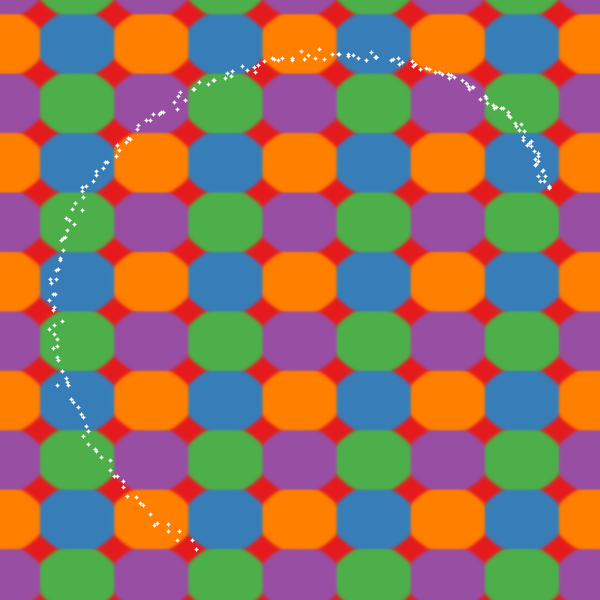
\includegraphics[clip, trim = 0cm 12cm 0cm 0.0cm, width=0.4\columnwidth]{../figures/hidden_bad} \\
Contours show $f(\vx)$,\\ a noise-tolerant representation \\ of a data manifold (white) %&
%A na\"{i}ve representation (colors) \\
\end{tabular}

\end{minipage}
&
\begin{minipage}[c]{0.6\columnwidth}
\begin{itemize}
\item { \color{mydarkblue} (Rifai et. al., 2011)} argue that a good latent representation is invariant in directions orthogonal to the manifold on which the data lie.  
\item Conversely, a good latent representation must also change in directions tangent to the data manifold, in order to preserve relevant information.
\end{itemize}
\end{minipage}
\end{tabular}



 
\mysection{Random deep nets have few degrees of freedom}

We visualize random mappings to show properties of prior on functions:
\vspace{0.3in}

\newcommand{\mappic}[1]{\hspace{-0.05in}\includegraphics[width=0.24\columnwidth]{../figures/map/latent_coord_map_layer_#1}} 
\newcommand{\mappiccon}[1]{\hspace{-0.05in}\includegraphics[width=0.24\columnwidth]{../figures/map_connected/latent_coord_map_layer_#1}}

\centering
\begin{tabular}{cccc}
Identity Map: $\vy = \vx$ & 1 Layer: $\vy = f^1(\vx)$ & 2 Layers: $\vy = f^{1:2}(\vx)$ & 40 Layers \\%\\2 Layers: $\vy = f_1(f_2(\vx))$ \\
\mappic{0} & \mappic{1} & \mappic{2} & \mappic{40}
\end{tabular}



\newcommand{\gpdrawbox}[1]{
\setlength\fboxsep{0pt}
\hspace{-0.36in} 
\fbox{
\includegraphics[width=0.23\columnwidth]{../figures/deep_draws/deep_gp_sample_layer_#1}
}}

As depth increases, there is usually only one direction we can move $\vx$ to change $\vy$.

\vspace{0.5in}
We also visualize a distribution warped by successive functions drawn from a \gpt{} prior:
\vspace{0.5in}

\centering
\begin{tabular}{cccc}
$p(\vx)$ & $p(\vf^{(1)}(\vx))$ & $p(\vf^{(1:4)}(\vx))$ &  $p(\vf^{(1:6)}(\vx))$ \\
\gpdrawbox{1} & \gpdrawbox{2} & \gpdrawbox{4} & \gpdrawbox{6} \\
\end{tabular}
As depth increases, the density concentrates along one-dimensional filaments.
\vspace{0.3in}



\newpage


\mysection{Fixing the pathology}

\begin{itemize}
	\item Following a suggestion from {\color{mydarkblue} (Neal, 1995)}, connect input to every layer:
\end{itemize}

\centering
%\def\layersep{1.33cm}
\def\nodeseptwo{1.8cm}
%\def\nodesize{.35cm}

%\newcommand{\numdims}[0]{3}
%\newcommand{\numhidden}[0]{4}
%\newcommand{\upnodedist}[0]{0.6cm}
%\newcommand{\bardist}[0]{\hspace{-0.2cm}}

\begin{tabular}{c}
\bardist
Standard architecture: \\
\begin{tikzpicture}[draw=black!80]
    \tikzstyle{neuron}=[circle,minimum size=17pt, draw = black!80, fill = white, thick]
    \tikzstyle{input neuron}=[neuron, fill=green!50];
    \tikzstyle{output neuron}=[neuron, fill=red!50];
    \tikzstyle{hidden neuron}=[neuron, fill=blue!50];
    \tikzstyle{pile} =[thick, ->, >=stealth', shorten <=7pt, shorten >=8pt];

    % Define the input layer node
    \coordinate (I) at (0, 0);


    % Define the hidden layer nodes
    \foreach \name / \i in {1,...,\numhidden}
    {
        \coordinate (H-\name) at (\nodeseptwo * \i, 0);
    }

    % Connect every node            
    \foreach \name in {1,...,\numhidden}
    {
	 \path[pile] (I) edge (H-\name) {};
         %\path[pile] (I) edge [bend left] (H-\name) {};
    }

    \draw (I) node[neuron] {};
    \draw (I) node[below = 0.5cm]  {$\vx$};

    % Draw the hidden layer nodes
    \foreach \name / \y in {1,...,\numhidden}
    {
	\draw (H-\name) node[neuron]  {};
        \draw (H-\name) node[below = 0.34cm] {$\vf^{(\y)}(\vx)$};
    }
\end{tikzpicture} \\
\vspace{\baselineskip}
\\
Input-connected architecture: \\
\bardist
\begin{tikzpicture}[draw=black!80]
    \tikzstyle{neuron}=[circle,minimum size=17pt, draw = black!80, fill = white, thick]
    \tikzstyle{input neuron}=[neuron, fill=green!50];
    \tikzstyle{output neuron}=[neuron, fill=red!50];
    \tikzstyle{hidden neuron}=[neuron, fill=blue!50];
    \tikzstyle{pile} =[thick, ->, >=stealth', shorten <=7pt, shorten >=8pt];

    % Define the input layer node
    \coordinate (I) at (0, 0);


    % Define the hidden layer nodes
    \foreach \name / \y in {1,...,\numhidden}
    {
        \coordinate (H-\name) at (\nodeseptwo*\y, 0);
    }

    % Connect every node            
    \path[pile] (I) edge (H-1) {};
    \foreach \name in {2,...,\numhidden}
    {
	 \path[pile] (I) edge (H-\name) {};
         \path[pile] (I) edge [bend left] (H-\name) {};
    }

    \draw (I) node[neuron] {};
    \draw (I) node[below = 0.5cm]  {$\vx$};

    % Draw the hidden layer nodes
    \foreach \name / \y in {1,...,\numhidden}
    {
	\draw (H-\name) node[neuron]  {};
        \draw (H-\name) node[below = 0.34cm] {$\vf^{(\y)}(\vx)$};
    }
\end{tikzpicture} 
\end{tabular}


%Two different architectures for deep neural networks.  The standard architecture connects each layer's outputs to the next layer's inputs.  The input-connected architecture connects also connects the original input $\vx$ to each layer.

\vspace{0.3in}

\begin{itemize}
	\item This fixes the problem:  Locally there are usually $D$ degrees of freedom, at any depth:
\end{itemize}
\vspace{0.3in}

\begin{tabular}{cccc}
Identity Map: $\vy = \vx$ & 2 connected Layers & 10 Connected Layers & 40 Connected Layers \\%\\2 Layers: $\vy = f_1(f_2(\vx))$ \\
\hspace{-0.07in} \mappic{0} & \mappiccon{2} & \mappiccon{10} & \mappiccon{40}
%\mappic{4} & \mappic{10} & \mappic{40} \\
%4 Layers & 10 Layers & 
\end{tabular}


\newcommand{\gpdrawboxcon}[1]{
\setlength\fboxsep{0pt}
\hspace{-0.4in} 
\fbox{
\includegraphics[width=0.47\columnwidth]{../figures/deep_draws_connected/deep_sample_connected_layer#1}
}}





\begin{tabular}{cc}
\begin{minipage}[c]{0.5\columnwidth}

Pathology is also resolved in deep density models:  Density does not concentrate along filaments when input connects to all layers.


\end{minipage}
&
\begin{minipage}[c]{0.5\columnwidth}
\centering
\begin{tabular}{cc}
%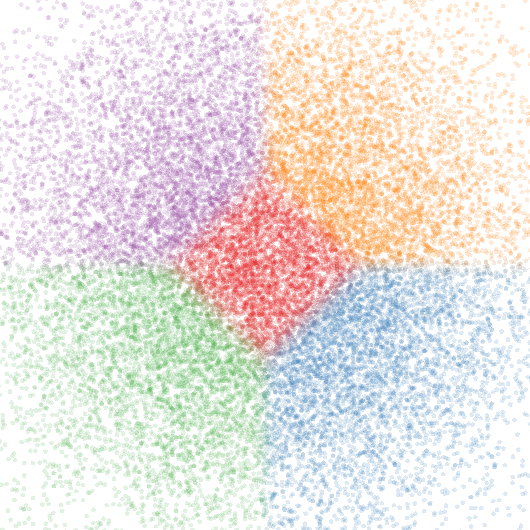
\includegraphics[width=0.3\columnwidth]{figures/deep_draws/deep_gp_sample_layer_1} &
%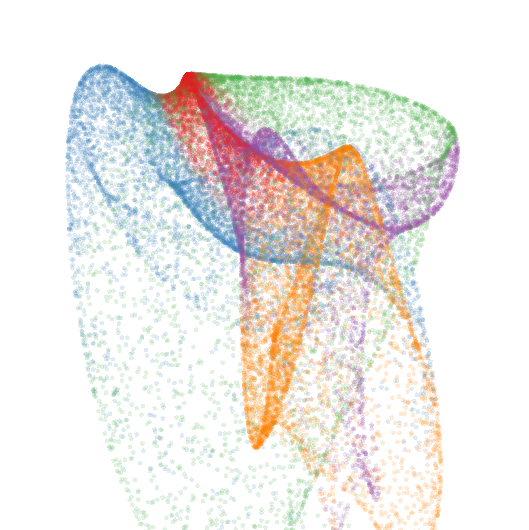
\includegraphics[width=0.3\columnwidth]{figures/deep_draws_connected/deep_sample_connected_layer2} &
%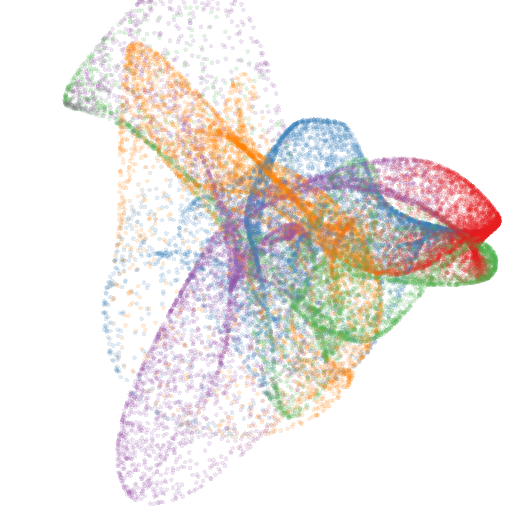
\includegraphics[width=0.3\columnwidth]{figures/deep_draws_connected/deep_sample_connected_layer3} \\
%$p(\vx)$ & $p(f_1(\vx))$ & $p(f_2(f_1(\vx), \vx))$ \\ \\
%\gpdrawboxcon{2} &
 4 Layers & 5 Layers \\
\gpdrawboxcon{4} &
\gpdrawboxcon{5}
\end{tabular}
\end{minipage}
\end{tabular}





\mysection{Explaining the Pathology}

\newcommand{\spectrumpic}[1]{
%\hspace{-0.2in}
\includegraphics[trim=5mm 0mm 4mm 6.4mm, clip, width=0.25\columnwidth]{../figures/spectrum/layer-#1}} 


\begin{tabular}{cc}
\begin{minipage}[c]{0.73\columnwidth}

%{\bf Theorem}
%The Jacobian of a deep \gp{} with a product kernel is a product of independent Gaussian matrices, with each entry in each matrix being drawn independently.

\begin{itemize}
\item Jacobian of a deep GP is a product of independent Gaussian matrices.
\item Singular values spectrum of Jacobian quantifies relative size of derivatives.
\item As the net gets deeper, distribution of SVs becomes heavy-tailed, and the largest singular value dominates.
\item Eventually, there is only one direction we can move $\vx$, in order to change $\vy$.
\end{itemize}

%Normalized singular value spectrum of the Jacobian of a deep GP.    This implies that with high probability, there is only one effective degree of freedom in the representation being computed.  As depth increases, the distribution on singular values also becomes heavy-tailed.

\end{minipage}
&
\begin{minipage}[c]{\columnwidth}
\begin{centering}
\begin{tabular}{ccc}
2 layer SV spectrum \\
\hspace{-0.16in} \spectrumpic{2} \\
%4 layers & 
6 layers SV spectrum \\
\hspace{-0.16in} \spectrumpic{6} 
%2 layers & 4 layers & 6 layers
\end{tabular}
\end{centering}
\end{minipage}
\end{tabular}



\mysection{Infinitely Deep Kernels}


\begin{minipage}[c]{0.6\columnwidth}

\begin{itemize}
\item Can also analyze fixed deep feature mappings:
\item {\color{mydarkblue} (Cho, 2012) } built kernels from multiple layers of feature mappings:
\item If ${k_1(\vx, \vx') = \Phi(\vx) \tra \Phi(\vx')}$, we can also build kernel ${k_2(\vx, \vx') = k_2(\Phi(\vx), \Phi(\vx')) = \Phi(\Phi(\vx)) \tra \Phi(\Phi(\vx'))}$.
%
%We can consider applying the feature transform $\Phi(\cdot)$ to the features themselves:  $\Phi_2 = \Phi(\Phi(\vx))$.  

\item For the squared-exp kernel, this composition operation has a closed form:% for any set of starting features $\Phi_n(\vx)$:
%
%In this section, we take the infinite limits of these compositions, and propose a new variant.
%
%One can derive a Gaussian process as a neural network: $f(x) = {\mathbf \alpha}^T \Phi(x) = \sum_{i=i}^K \alpha_i \phi_i(x)$.  
%
%
%we derive a kernel which corresponds to arbitrarily many compositions of the feature vectors corresponding to the squared-exp kernel:
%
\begin{align*}
%k_1(\vx, \vx') & = \exp \left( -\frac{1}{2} ||\vx - \vx'||_2^2 \right) \\
& k_{n+1}(\vx, \vx') = \nonumber \\
& = \exp \left( -\frac{1}{2} \left|\left| \left[ \! \begin{array}{c} \Phi_n(\vx) \\ \vx \end{array} \! \right]  - \left[ \! \begin{array}{c} \Phi_n(\vx') \\ \vx' \end{array} \! \right] \right| \right|_2^2 \right) \nonumber \\
%k_{n+1}(\vx, \vx') 
%& = \exp \left( -\frac{1}{2} \sum_i \left[ \phi_i(\vx) - \phi_i(\vx') \right]^2 -\frac{1}{2} || \vx - \vx' ||_2^2 \right) \\
%k_{n+1}(\vx, \vx') & = \exp\left ( -\frac{1}{2} \sum_i \left[ \phi_i(\vx)^2 - 2 \phi_i(\vx) \phi_i(\vx') + \phi_i(\vx')^2 \right]  -\frac{1}{2} || \vx - \vx' ||_2^2 \right) \\
%k_2(\vx, \vx') & = \exp \left( -\frac{1}{2} \left[ \sum_i \phi_i(\vx)^2 - 2 \sum_i \phi_i(\vx) \phi_i(\vx') + \sum_i \phi_i(\vx')^2 \right] \right) \\
%k_2(\vx, \vx') & = \exp \left( -\frac{1}{2} \left[ k_1(\vx, \vx) - 2 k_1(\vx, \vx') + k_1(\vx', \vx') \right] \right) \\
%k_{n+1}(\vx, \vx') 
& = \exp \left( k_n(\vx, \vx') - 1 -\frac{1}{2} || \vx - \vx' ||_2^2 \right)
\end{align*}

\item This kernel satisfies $k_\infty - \log(k_\infty) = 1 + \frac{1}{2} || \vx - \vx' ||_2^2$
\item No closed form, but it is continuous and differentiable everywhere except at $\vx = \vx'$.
\end{itemize}
\end{minipage}
\begin{minipage}[c]{0.39\columnwidth}
\begin{centering}
\begin{tabular}{c}
%\hspace{-0.5cm}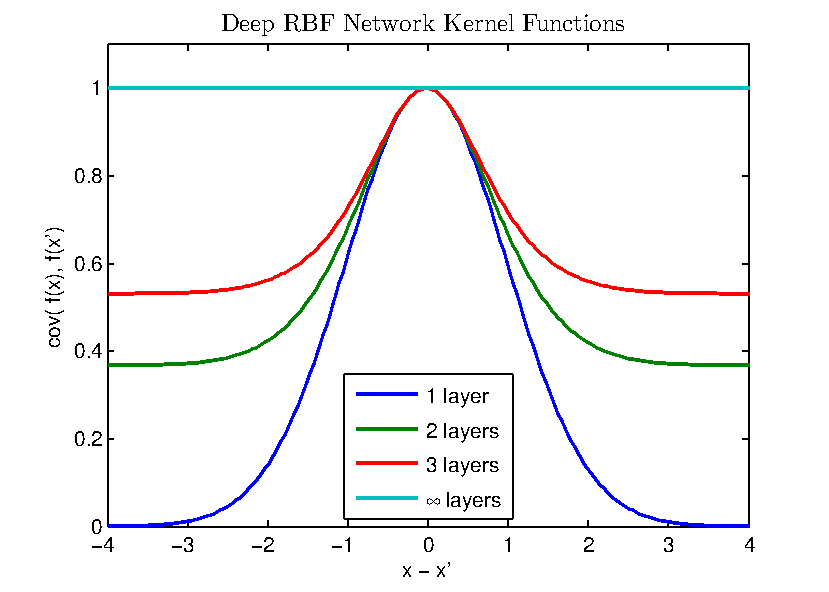
\includegraphics[width=0.33\columnwidth, clip, trim = 0cm 0cm 1cm 0.61cm]{../figures/deep_kernel} &
deep connected kernel \\
\hspace{-0.5cm}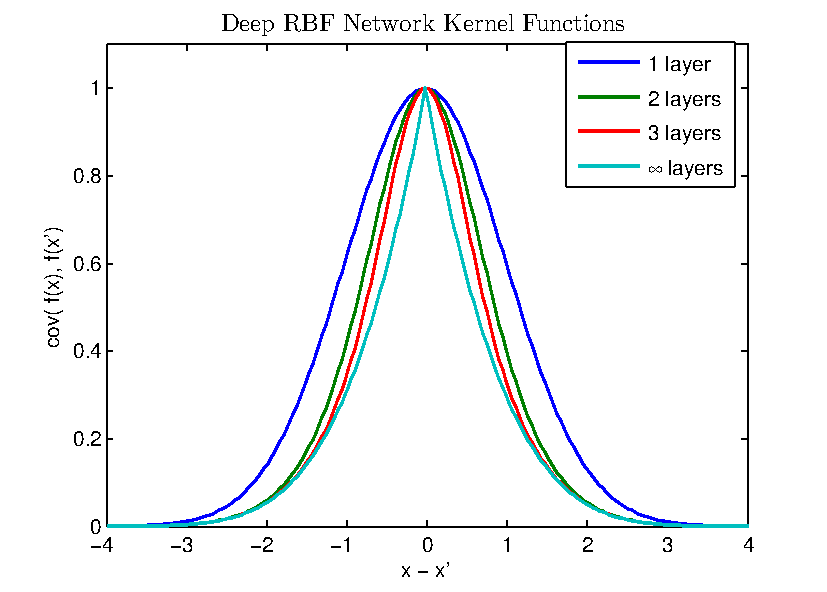
\includegraphics[width=\columnwidth, clip, trim = 0cm 0cm 1cm 0.61cm]{../figures/deep_kernel_connected} \\
Connected \gp{} draws \\
\hspace{-0.5cm}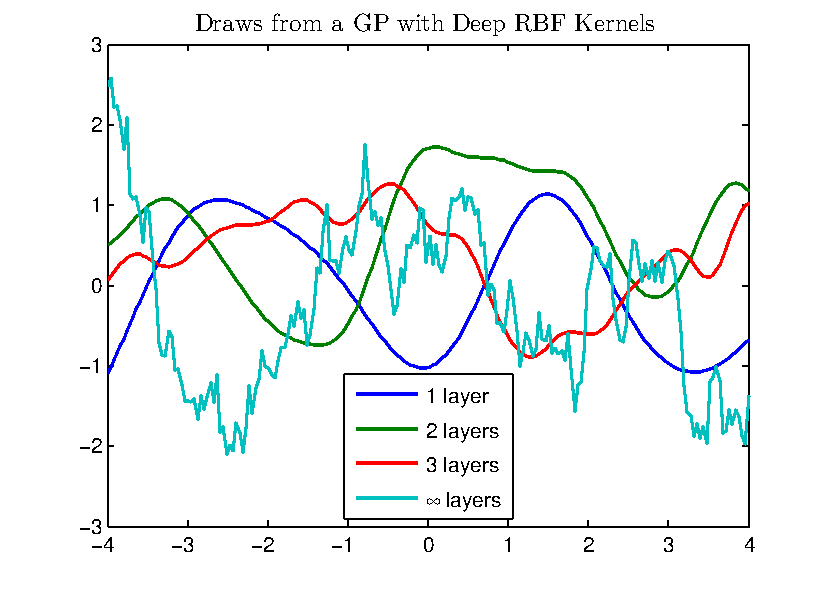
\includegraphics[width=\columnwidth, clip, trim = 0cm 0cm 1cm 0.61cm]{../figures/deep_kernel_connected_draws}
\end{tabular}
\end{centering}
\end{minipage}








\mysection{Conclusions}
\begin{itemize}
	\item Random networks capture fewer degrees of freedom as they get deeper
	\item Connecting the input to each layer resolves this pathology
	\item Deep Gaussian processes are a data-independent way to characterize neural networks
	\item Deep One-Dimensional GPs have a log-normal distribution on the magintude of their derivatives.
	\item Can build ``deep net'' kernels
\end{itemize}


\raggedright

\begin{tabular}{cc}
\begin{minipage}[c]{0.8\columnwidth}

Code at \texttt{github.com/duvenaud/deep-limits}

Paper at \texttt{mlg.eng.cam.ac.uk/duvenaud/papers/verydeep.pdf}

\end{minipage}
&
\begin{minipage}[c]{0.2\columnwidth}
\begin{centering}

\includegraphics[width=\linewidth]{figures/qrcode-paper-link}
\end{centering}
\end{minipage}
\end{tabular}
%
%
%
\end{multicols}
\end{poster}

\end{document}

